% PLE-SBS research poster (A0 landscape). Build: cd poster && tectonic PLESBS_Poster.tex
% Figures: ../figures (paper figures), ../cad (rig drawings), img/ (poster-only panels from make_poster_figs.py)
\documentclass[20pt, a0paper, landscape, margin=0mm, innermargin=14mm, blockverticalspace=8mm, colspace=12mm, subcolspace=8mm]{tikzposter}
\usepackage[utf8]{inputenc}
\usepackage[T1]{fontenc}
\usepackage{lmodern}
\usepackage{amsmath, amssymb}
\usepackage{graphicx}
\usepackage{booktabs}
\usepackage{enumitem}
\setlist{nosep, leftmargin=1.2em}
\graphicspath{{../figures/}{../cad/}{img/}{../scale_down/}}

\definecolor{padnavy}{RGB}{24,40,58}
\definecolor{padorange}{RGB}{228,87,14}
\definecolor{padgrey}{RGB}{244,246,248}
\definecolorstyle{PadStyle}{
  \colorlet{colorOne}{padnavy}
  \colorlet{colorTwo}{padorange}
  \colorlet{colorThree}{padgrey}
}{
  \colorlet{backgroundcolor}{white}
  \colorlet{framecolor}{white}
  \colorlet{titlefgcolor}{white}
  \colorlet{titlebgcolor}{colorOne}
  \colorlet{blocktitlebgcolor}{colorOne}
  \colorlet{blocktitlefgcolor}{white}
  \colorlet{blockbodybgcolor}{colorThree}
  \colorlet{blockbodyfgcolor}{black}
  \colorlet{innerblocktitlebgcolor}{colorTwo}
  \colorlet{innerblocktitlefgcolor}{white}
  \colorlet{innerblockbodybgcolor}{white}
  \colorlet{innerblockbodyfgcolor}{black}
  \colorlet{notefgcolor}{black}
  \colorlet{notebgcolor}{white}
  \colorlet{noteframecolor}{colorTwo}
}
\usetheme{Default}
\usecolorstyle{PadStyle}
\useblockstyle{Basic}
\tikzposterlatexaffectionproofoff
\usetitlestyle{Filled}

\title{\parbox{0.95\linewidth}{\centering PLE-SBS: a way down from a fuelled rocket, with the power off, in two minutes}}
\author{Adithya Kesan Jayakanth \quad\textbar\quad adithya.kesan@icloud.com \quad\textbar\quad Mentor and guide: Mrs.\ Abhitha Peter}
\institute{A slidewire basket escape system and a sizing rule for any launch pad. Grade 12, Padma Seshadri Bala Bhavan Senior Secondary School, K.K.~Nagar, Chennai. Paper, 6 July 2026. Simulator: adithyakesan.com/ple\_sbs}

\begin{document}
\maketitle[width=0.98\textwidth]

\begin{columns}

%%%%%%%%%%%%%%%%%%%%%%%%%%%%%%%%%%%%%%%%%%%%%%%%%%%%%%%%%%%%%%%% column 1
\column{0.24}

\block{1 \, Where this came from}{
\textbf{A roller coaster is a machine for giving people forces safely.} In an earlier paper I designed coaster tracks under human g and jerk limits. The lesson that stuck: the thrill and the limit are the same number. The ride is good \emph{because} it runs close to what a body can take, and safe because it never crosses that line.

\vspace{3mm}
\textbf{A visit to ISRO turned the same idea toward crewed launch.} In the hours before lift-off, astronauts and close-out technicians work 40--115\,m up a tower beside a fully fuelled rocket. If something goes wrong they need a way down that beats the lifts, works with the power off and keeps working in a storm. NASA uses gravity-driven slidewire baskets, each engineered for one pad.

\vspace{3mm}
\textbf{So this is a coaster designed for the worst day instead of the best one.} Gravity drives it, a brake limits it, 1.5\,g is the line it must not cross, and the only score is how fast the last person is behind a blast door.

\vspace{4mm}
\innerblock{The questions}{
\begin{itemize}
  \item Can one \textbf{method} size a slidewire for \emph{any} rocket on \emph{any} pad?
  \item What makes the design \textbf{fail}, and what is left once the hardware works?
  \item Can every pod share \textbf{one wire} and still stop safely if a brake fails?
\end{itemize}
}
\vspace{3mm}
\textbf{How I worked.} The same loop each round: write down who needs what as requirements; design the physics on paper; build something that runs; run it until it breaks; put the failure back into the design. Five rounds of that loop are the spine of this poster.
}

\block{2 \, The problem, bounded}{
\textbf{Scenario:} alarm; crew unstrap and leave the capsule (60\,s); walk the access arm; board; ride; leave the pod; reach shelter. The clock stops when the \emph{last} person is protected. Worked example: 3 crew + 6 technicians on a low 42\,m pad.

\vspace{3mm}
\begin{tabular}{@{}cp{0.83\linewidth}@{}}
\toprule
R1 & Everyone protected within the window, at P95 not the average \\
R2 & No electrical power: gravity drive, passive brakes \\
R3 & Works in 17.5\,m/s (34\,kn) along-wire wind, either direction \\
R4 & Peak deceleration $\le 1.5$\,g, seated and belted \\
R5 & No stalls, no pod within 5\,m of another, dock cleared first \\
R6 & Rope tension $\le$ breaking strength\,/\,5 \\
R7 & Terminus outside the fireball; shelter rated for the blast there \\
\bottomrule
\end{tabular}

\vspace{3mm}
Five illustrative \textbf{danger levels} (my assumptions) set how much propellant joins an explosion and how long the warning is. Level 4, a pad fire, has a 120\,s window, the Shuttle-era two-minute requirement.
}


\block{3 \, The 1:50 printed model}{
\begin{center}
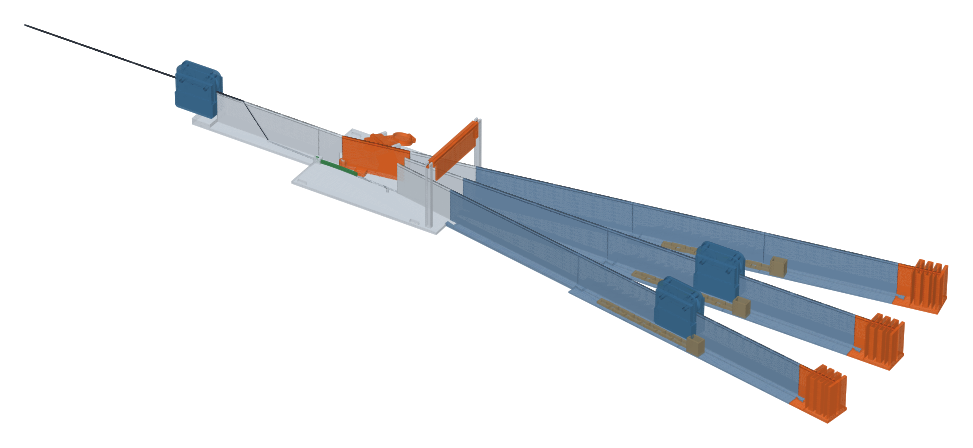
\includegraphics[width=0.70\linewidth]{render_yard.png}
\end{center}
\vspace{-3mm}
Only the 1.5\,mm wire is bought; 26 printed parts make the rest, including block 8's switch yard in miniature. Each passing pod lifts a flap that rocks a two-finger escapement, and a spring steps the tongue to the next bay: 1, 2, 3 in turn. A printed comb, chain and bumper stop the pods.
}

%%%%%%%%%%%%%%%%%%%%%%%%%%%%%%%%%%%%%%%%%%%%%%%%%%%%%%%%%%%%%%%% column 2
\column{0.24}

\block{4 \, Designing the physics}{
\textbf{How far is far enough?} Propellant becomes an equivalent mass of TNT (DoD rules; my own 10--20\,\% for hypergolics and methane). Blast distance scales as $R = 40\,W^{1/3}$ (1.2\,psi). Fireball diameter and duration follow $D = 3.86 M^{0.32}$\,m, $t = 0.30 M^{0.32}$\,s, and a person is safe when the thermal dose $q^{4/3}t$ stays below 100\,(kW/m$^2$)$^{4/3}$s. Reference launcher, level 4: 17.2\,t TNT, blast 409\,m, a 172\,m fireball for 13\,s, so \textbf{573\,m} is required.

\begin{center}
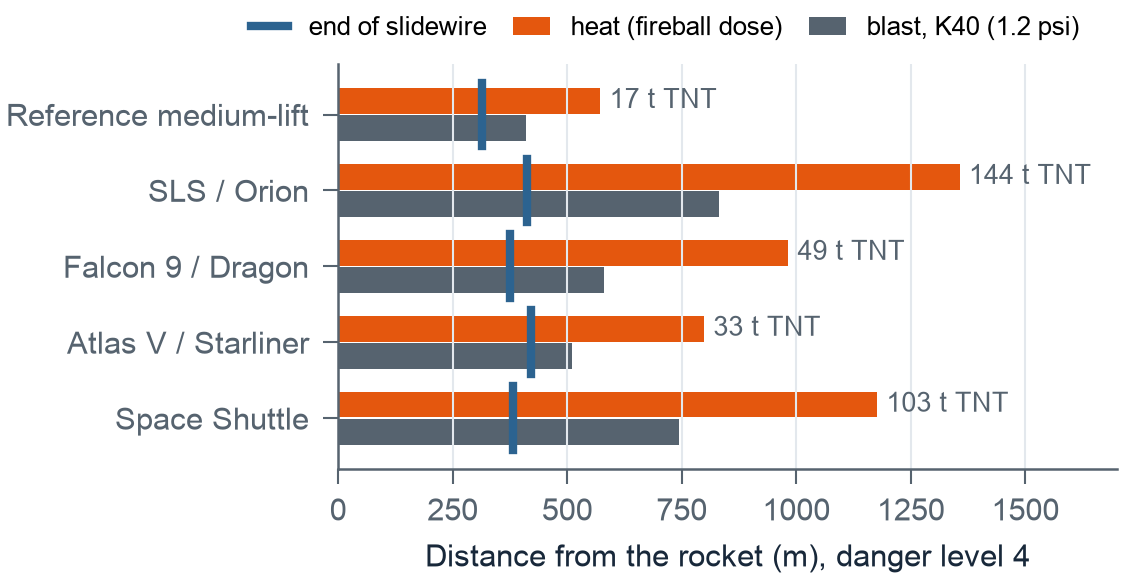
\includegraphics[width=0.72\linewidth]{fig2_hazard.png}
\end{center}
\vspace{-2mm}
Heat sets the distance for every vehicle, and \textbf{every real slidewire ends inside it}. The wire is the first leg; a bunker or an armoured vehicle finishes the job.

\vspace{3mm}
\textbf{The wire is not straight, and the pods are coupled.} A taut string at constant tension sags under its own weight and under every pod. A pod behind \emph{lifts} the wire under the pod ahead and can flatten its final approach until it stalls, so all pods on a wire are integrated together. Worked example: 36\,mm rope at 150\,kN sags 4.1\,m; peak tension 154\,kN against 181\,kN allowed.

\vspace{3mm}
\textbf{The ride and the brake.} Each pod obeys
\[
m\dot v = mg\sin\theta - \mu mg\cos\theta - \tfrac12\rho C_dA\,(v-u\cos\theta)|v-u\cos\theta| - k_b v,
\]
the last term a passive eddy-current brake. Its deceleration is $k_b v/m$, so \textbf{a light pod is braked harder than a heavy one}. I size $k_b$ at two corners: a full pod in a 17.5\,m/s tailwind must dock at $\le 4$\,m/s; the lightest pod in a 17.5\,m/s headwind must never drop below 1\,m/s. When they conflict, the light pod wins and a catch net takes what the magnets cannot.
}

\block{5 \, Building it, and checking it against NASA}{
\begin{itemize}
  \item \textbf{One physics file} (about 870 lines of dependency-free JavaScript) runs the website \emph{and} produces every number and figure in the paper, so the paper cannot drift from the model.
  \item \textbf{Sixteen unit tests} against closed-form cases: $\sqrt{2gh}$ arrival, terminal speed, $wL^2/8T$ and $PL/4T$ sag, the chain-bed stop in $v/\omega$, a stalled pod holding the one behind it. Halving the 0.02\,s step moves the answer by 0.03\,s.
  \item \textbf{Web simulator:} any rocket on any pad, dock or switch yard, net or chain bed, a brake you can fail. It animates the pods on the sagging wires with the hazard rings to scale and checks R1--R7. Works offline and on a phone.
  \item \textbf{Validation, no tuning.} Shuttle LC-39B (59\,m drop, 362\,m span): predicted peak 24.0\,m/s against the reported ``approximately 55\,mph'' (24.6\,m/s), within 3\,\%. Artemis (114\,m drop): gravity alone gives 77\,mph against the reported 40--55\,mph; a 300\,m braked section holds it to 55\,mph, so on a tall tower the magnets must act over much of the descent. Block 7 shows this is a general rule.
\end{itemize}
}

%%%%%%%%%%%%%%%%%%%%%%%%%%%%%%%%%%%%%%%%%%%%%%%%%%%%%%%%%%%%%%%% column 3
\column{0.28}

\block{6 \, Running it until it broke: five redesigns}{
Each row is a full evacuation of 9 people at level 4, at both wind corners, and 1,000 times in Monte Carlo. Each problem found by \emph{running} the system went back into the design.

\vspace{2mm}
\begin{tabular}{@{}cp{0.49\linewidth}cccc@{}}
\toprule
 & Change & Time & P95 & Failing & Worst stop \\
\midrule
D0 & Copy Artemis: 400\,m, 1 wire $\times$ 3 pods in series, vehicle pick-up & 203\,s & 231\,s & 93\,\% & 16.4\,g \\
D1 & 2 wires $\times$ 2 pods, balanced loading & 184\,s & 213\,s & 91\,\% & 16.4\,g \\
D2 & 300\,m span into a 3\,m pit; light brake + 10\,m catch net & 188\,s & 218\,s & 0\,\% & 1.4\,g \\
D3 & Bunker 40\,m from the dock instead of a vehicle & 160\,s & 192\,s & 0\,\% & 1.4\,g \\
D4 & Crew pod at the arm exit, open pods, faster unload & \textbf{129\,s} & \textbf{162\,s} & 0\,\% & 1.4\,g \\
\bottomrule
\end{tabular}

\vspace{3mm}
\textbf{D0 is the whole difficulty in one row.} From only 42\,m of height a 400\,m wire ends almost flat. Any magnetic brake strong enough to matter strands a light pod in a headwind, so the auto-sizing chooses no brake, and a full pod in a tailwind hits the end at 25\,m/s. Going parallel (D1) fixes nothing. \textbf{Geometry fixed it} (D2): shorter, steeper, into a pit, with a long-stroke net. D3 and D4 then attacked what was left, which was people.

\vspace{2mm}
\begin{center}
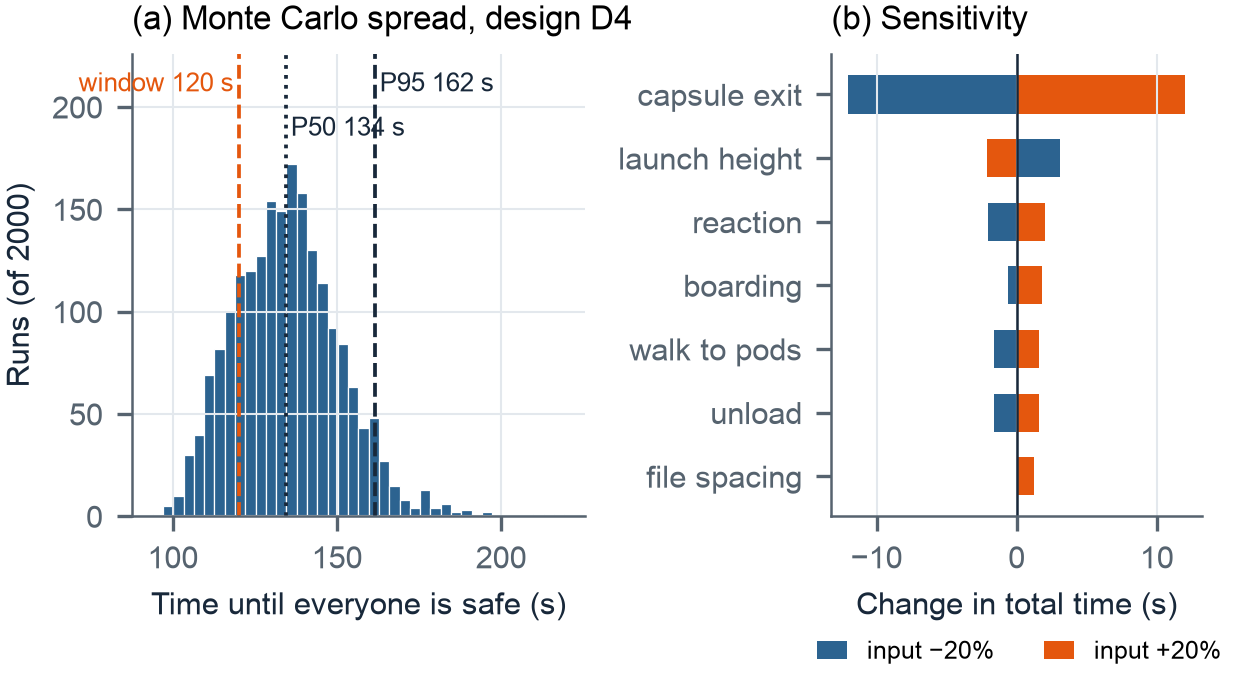
\includegraphics[width=0.78\linewidth]{mc_sensitivity.png}
\end{center}
\vspace{-2mm}
Fourteen inputs varied together over 2,000 runs: median 134\,s, P95 162\,s, 3 runs flagged. D4 meets levels 1--3 at P95 but \textbf{not} the 120\,s of level 4. The sensitivity says why: $\pm 20\,\%$ on capsule exit moves the total by $\pm 12$\,s, more than every hardware parameter combined. The crew reach the platform 78\,s after the alarm, before any wire can help them.
}

\block{7 \, A sizing rule for any pad}{
\begin{center}
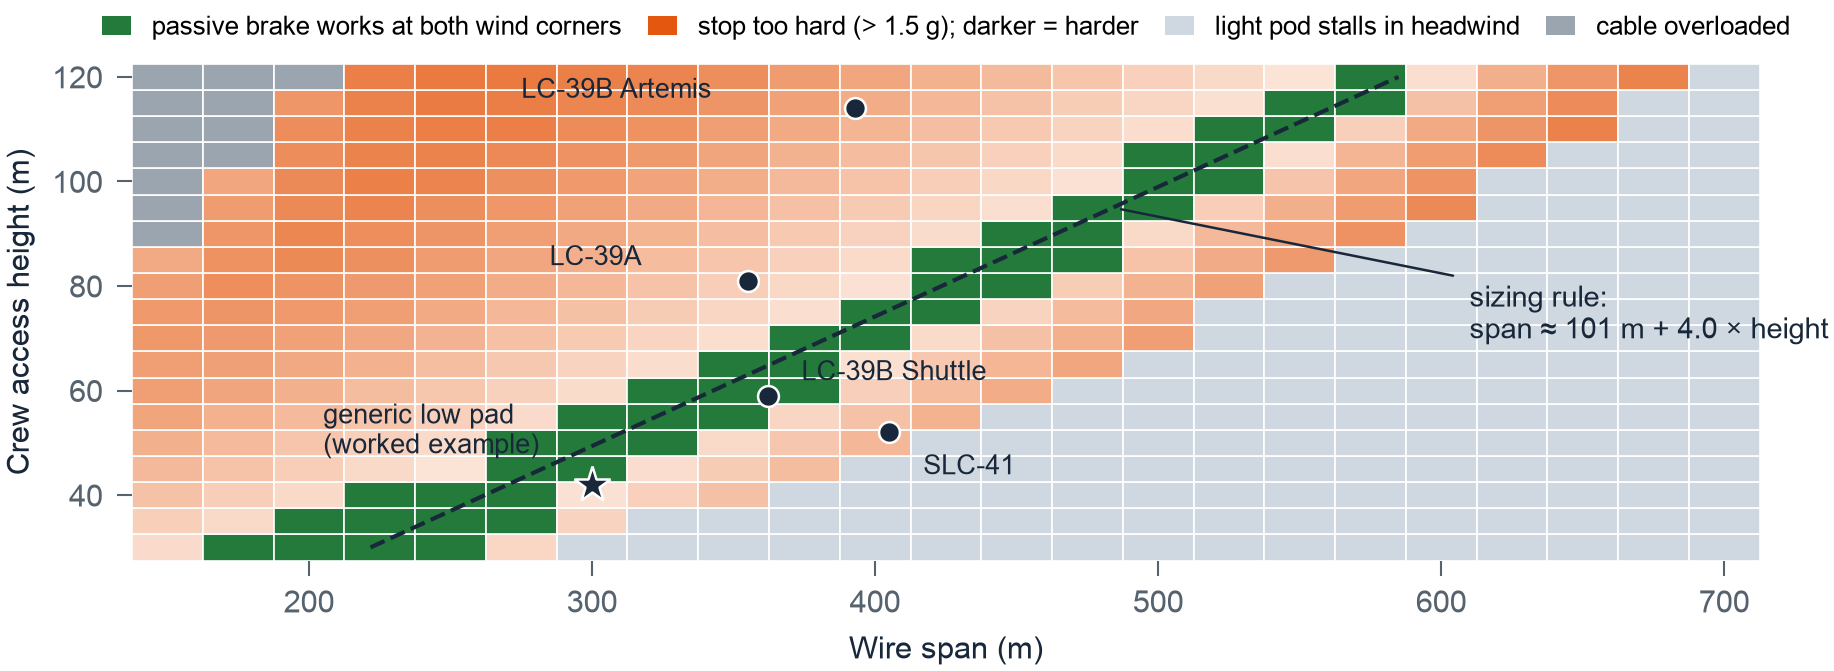
\includegraphics[width=0.86\linewidth]{fig4_feasibility.png}
\end{center}
\vspace{-2mm}
The two-corner brake check for every crew height 30--120\,m and span 150--700\,m. Passive braking works only in a \textbf{narrow diagonal band}: left of it the stop exceeds 1.5\,g, right of it a light pod stalls in a headwind. A line through the band gives $L_\text{span} \approx 100\ \text{m} + 4\,H_\text{crew}$, a slope of about 1 in 7 to 1 in 5. Existing pads sit where their braking choices predict: Shuttle (passive nets and chains) on the band; LC-39A and Artemis on the steep side, where Artemis indeed brakes along the line; SLC-41 on the flat side, where riders control their own brakes. The band is 25--75\,m wide, so the rule is a first cut and the simulator does the rest.
}

%%%%%%%%%%%%%%%%%%%%%%%%%%%%%%%%%%%%%%%%%%%%%%%%%%%%%%%%%%%%%%%% column 4
\column{0.24}

\block{8 \, My add-on: one wire, a switch yard, a bay per pod}{
Existing systems give every basket its own wire and brake it at the end of that wire. In D4 that shared end is the bottleneck: each pod crawls through the brake zone, stops, unloads and is cleared before the next may arrive, a 37\,s headway. D5 moves all of that \textbf{off the wire}.

\begin{center}
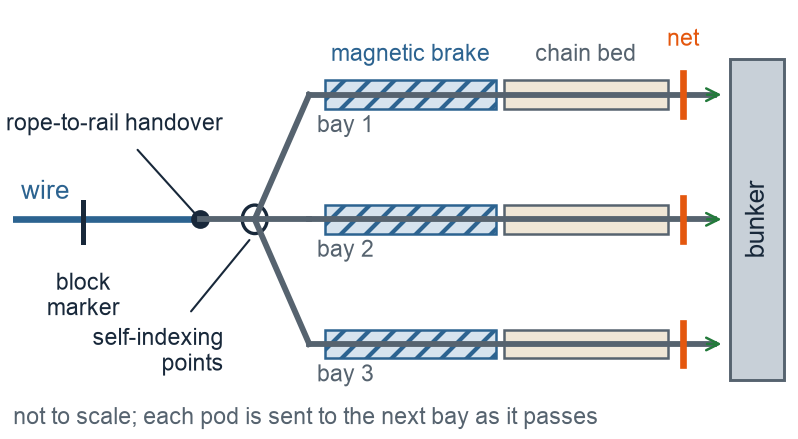
\includegraphics[width=0.70\linewidth]{fig7_switchyard.png}
\end{center}
\vspace{-2mm}
\begin{itemize}
  \item \textbf{Self-indexing points}, a turnout advanced by a ratchet each passing pod trips, send pod 1 to bay 1, pod 2 to bay 2. No power, no sensors.
  \item Each bay has a 60\,m magnetic brake, a \textbf{drag-chain bed} (force grows with distance, not speed, so the stop is simple-harmonic) and a backup net, 15\,m from the bunker door.
  \item \textbf{Release from inside} by a lever the occupants pull. A \textbf{block marker} on the wire, as in railway signalling, keeps it locked until the pod ahead is 60\,m down; a stalled pod holds the next one at the platform.
\end{itemize}
\vspace{2mm}
\innerblock{What it buys}{
\begin{itemize}
  \item Pods leave about \textbf{8\,s apart} instead of 37\,s.
  \item 24 people in six pods: \textbf{113\,s} on one wire in a design headwind, against 286\,s with a single dock and 111\,s with six separate wires.
  \item A pod whose brake has \textbf{failed} stops at 1.40\,g (1.76\,g with a tailwind), where D4's catch net gave 3.8\,g.
  \item Nine people: 131\,s, P95 162\,s, no failures in 1,000 runs, with one rope, one counterweight and one anchor.
\end{itemize}
}
}

\block{9 \, What I learned}{
\begin{itemize}
  \item \textbf{Design a safety system at its corners.} Nothing was decided by the average case, everything by the light pod in a headwind and the full pod in a tailwind.
  \item \textbf{The thrill and the limit are still the same number.} Passive braking is a band, not a knob: too little strands people, too much hurts them.
  \item \textbf{Running it is how you find out.} D0 looked like a sensible copy of a real system until it was operated: 93\,\% failure.
  \item \textbf{People, not pods, set the time.} Once the hardware worked, the remaining seconds were in the hatch, the arm and the boarding.
\end{itemize}
}

\block{10 \, Honest limits and next steps}{
\begin{itemize}
  \item No debris, basket sway or rope stretch. The launcher is a generic reference vehicle; danger levels and pad dimensions are my estimates; the hazard correlations are screening tools, not siting standards.
  \item One wire is one point of failure: a jammed trolley blocks everyone behind it, so crewed flights get a second wire as a backup. In the last minute before an explosion only the capsule's launch-escape system is fast enough.
  \item Next: timed runs on the printed model to fit $\mu$ and $C_dA$, model sway, test the rule on a real pad.
\end{itemize}
}

\end{columns}
\end{document}
